\id{ҒТАМР 52.47.15}{}

\begin{articleheader}
\sectionwithauthors{Н.А. Бесбаева, Г.Ж. Бимбетова, К.С. Надиров, М.Қ. Жантасов, Н.Ш. Отарбаев}{БҰРҒЫЛАУ ЕРІТІНДІСІНІҢ СІҢІРІЛУІН ТӨМЕНДЕТУГЕ АРНАЛҒАН ЖЕҢІЛДЕТІЛГЕН ПОЛИМЕРЛІ ҚҰРАМ}

{\bfseries
Н.А. Бесбаева,
Г.Ж. Бимбетова\textsuperscript{\envelope },
К.С. Надиров,
М.Қ. Жантасов,
Н.Ш. Отарбаев
}
\end{articleheader}

\begin{affiliation}
М.Әуезов атындағы Оңтүстік Қазақстан университеті, Шымкент, Қазақстан

\raggedright \textsuperscript{\envelope } Корреспондент-автор: \href{mailto:gulmnaz@mail.ru}{}
\end{affiliation}

Ұңғымаларды бұрғылау кезінде бұрғылау ерітіндісінің сіңірілуі кеуекті
немесе жарықшақты қабаттардың ашық болуымен байланысты. Сіңірілу
технологиялық себептерге немесе тау жыныстарының жатыс пішіндерінің
геологиялық жағдайларына байланысты болуы мүмкін. Геологиялық
себептер-сіңірілу қабатының түрі, қуаты мен оның жатыс пішінінің
тереңдігі, гидравликалық жарылысқа тау жыныстарының төзімділігінің
жеткіліксіздігі, қабат қысымы және қабат сұйықтығының сипаттамасы,
сонымен бірге, басқа да ілеспе қиындықтардың болуы (опырылуы,
мұнайгаздың пайда болуы, қабат суларының ағындары және т.б.). Болатын
технологиялық себептерге ұңғымаға айдалатын бұрғылау ерітіндісінің саны
мен сапасы, бұрғылау әдісі, көтеріп-түсіру операцияларын жүргізу
жылдамдығы және техникалық жабдықтау, бұрғылау процесін ұйымдастыру
сияқты факторлар кіреді.

Берілген мақалада ұңғымадағы бұрғылау ерітіндісінің тау жыныстарының
жарықшақтарына сіңірілуін төмендету мүмкіндігі мен пайда болу мәселелері
қарастырылды. Ерітіндінің сіңірілуін төмендетудің қолданыстағы әдістері
талданды және қиын жағдайларда сәтті бұрғылауды жүзеге асыру бойынша
ұсыныстар жасалды.

Сонымен қатар, мақалада әр түрлі мөлшердегі қатынаста модификацияланған
полиакриламид пен ұсақталған мақта талшығының бұрғылау ерітіндісінің
қасиеттеріне әсері туралы зерттеу нәтижелері келтірілген. Бұл зерттеулер
ұңғыма қабырғасының қабықшалы қабат арқылы бұрғылау ерітіндісінің
сіңірілу жылдамдығын төмендету мақсатында жүргізілді. Модификацияланған
полиакриламид пен ұсақталған мақта талшығының концентрациясының бұрғылау
ерітіндісінің реологиялық қасиеттерінің көрсеткіштеріне (ығысудың
статикалық кернеуі және шартты тұтқырлық) әсері бойынша зерттеулер
жүргізілді. Құрамында бентонит сазы бар жеңілдетілген бұрғылау
ерітіндісіне ұсақталған мақта талшығын енгізу тұтқырлықты жоғарылатады
және судың бергіштігін төмендетеді, сонымен қатар ұңғыма қабырғасына
сапалы қабықшаның пайда болуына ықпал етеді. Осылай, ерітіндінің негізгі
көрсеткіштер бойынша оң нәтиже көрсеткен оңтайлы құрам анықталды, бұл
авторлардың пікірінше, мұнайгаз ұңғымаларын бұрғылау кезінде сіңірілетін
ерітіндінің көлемін төмендетуге ықпал етеді.

{\bfseries Түйін сөздер:} мұнай, бұрғылау ерітіндісі, мақта талшығы,
полиакриламид, май қышқылы, госсипол шайыры, полимерлі бұрғылау
ерітіндісі, каустикалық сода, ерітіндінің сіңірілуі, сіңірілуді
төмендету.

\begin{articleheader}
{\bfseries ПОЛИМЕРНЫЙ СОСТАВ ДЛЯ СНИЖЕНИЯ ПОГЛОЩЕНИЯ БУРОВОГО РАСТВОРА}

{\bfseries
Н.А. Бесбаева,
Г.Ж. Бимбетова\textsuperscript{\envelope },
К.С. Надиров,
М.Қ. Жантасов,
Н.Ш. Отарбаев
}
\end{articleheader}

\begin{affiliation}
Южно-Казахстанский университет им. М. Ауэзова, Шымкент, Казахстан,

e-mail: \href{mailto:gulmnaz@mail.ru}{}
\end{affiliation}

Поглощения бурового раствора при бурении скважин связано с вскрытием
пористых или трещиноватых пластов. Поглощения могут быть вызваны
технологическими причинами или геологическими условиями залегания горных
пород. Геологические причины - тип поглощающего пласта, его мощность и
глубина залегания, недостаточность сопротивления пород гидравлическому
разрыву, пластовое давление и характеристика пластовой жидкости, а также
наличие других сопутствующих осложнений (обвалы,
нефтегазоводопроявления, перетоки пластовых вод и др.). Технологические
причины - количество и качество подаваемого в скважину бурового
раствора, способ бурения, скорость проведения спускоподъемных операций и
другие. К этой группе относятся такие факторы, как техническая
оснащенность и организация процесса бурения.

Рассмотрены вопросы возникновения и возможности снижения поглощений
бурового раствора в скважине. Проанализированы существующие методы
снижения поглощения раствора и сформулированы рекомендации для
реализации успешного бурения в осложненных условиях.

В данной статье приведены результаты исследований по влиянию
модифицированного полиакриламида, а также измельченного хлопкового
волокна в различных соотношениях на свойства бурового раствора. Данные
исследования проведены с целью снижения скорости поглощения бурового
раствора через корковый слой стенки скважины. Проведены исследования по
влиянию концентрациимодифицированного полиакриламида и измельченного
хлопкового волокна на реологические показатели бурового раствора
(статическое напряжение сдвига и условная вязкость). Показано, что
введение измельченного хлопкового волокна в состав облегченного бурового
раствора, содержащего бентонитовой глину, приводит к повышению вязкости
и одновременно снижает водоотдачу, а также способствует образованию
качественной корки стенки скважины.

Таким образом, выявлен оптимальный состав раствора, который показал
положительные результаты по основным показателям, что, по мнению
авторов, будет способствовать снижению объема поглощаемого раствора при
бурении нефтегазовых скважин.

{\bfseries Ключевые слова:} нефть, буровой раствор, хлопковые волокна,
полиакриламид, жирные кислоты, госсиполовая смола, полимерные буровые
растворы, каустическая сода, поглащения раствора, снижение поглащении.

\begin{articleheader}
{\bfseries POLYMER COMPOSITION TO REDUCE THE ABSORPTION OF DRILLING MUD}

{\bfseries
N.A. Besbaeva,
G.ZH. Bimbetova\textsuperscript{\envelope },
K.S. Nadirov,
M.K. Zhantasov,
N.Sh. Otarbaev
}
\end{articleheader}

\begin{affiliation}
M.Auezov South Kazakhstan State University, Shymkent, Kazakhstan,

e-mail: \href{mailto:gulmnaz@mail.ru}{}
\end{affiliation}

The absorption of drilling mud during well drilling is associated with
the opening of porous or fractured formations. Uptake may be caused by
technological reasons or geological conditions of rock occurrence.
Geological reasons are the type of absorbing formation, its thickness
and depth of occurrence, insufficient rock resistance to hydraulic
fracturing, reservoir pressure and characteristics of reservoir fluid,
as well as the presence of other concomitant complications (landslides,
oil and gas occurrences, overflows of reservoir waters, etc.). The
technological reasons are the quantity and quality of drilling mud
supplied to the well, the drilling method, the speed of descent
operations, and others. This group includes factors such as technical
equipment and organization of the drilling process.

The issues of the occurrence and the possibility of reducing the
absorption of drilling mud in the well are considered. The existing
methods of reducing the absorption of the solution are analyzed and
recommendations are formulated for the implementation of successful
drilling in complicated conditions.

This article presents the results of studies on the effect of modified
polyacrylamide, as well as crushed cotton fiber in various ratios on the
properties of drilling mud. These studies were conducted in order to
reduce the rate of absorption of drilling mud through the cortical layer
of the well wall. Studies have been conducted on the effect of the
concentration of modified polyacrylamide and crushed cotton fiber on the
rheological parameters of the drilling mud (static shear stress and
conditional viscosity). It is shown that the introduction of crushed
cotton fiber into the composition of a lightweight drilling mud
containing bentonite clay leads to an increase in viscosity and at the
same time reduces water loss, as well as contributes to the formation of
a high-quality crust of the well wall.

Thus, the optimal composition of the solution was identified, which
showed positive results in terms of the main indicators, which,
according to the authors, will contribute to reducing the volume of
absorbed solution when drilling oil and gas wells.

{\bfseries Keywords:} oil; drilling mud; cotton fibers;
polyacrylamide; fatty acids; gossypol resin; polymer drilling fluids;
caustic soda; absorption of the solution; reduction of absorption.

\begin{multicols}{2}
{\bfseries Кіріспе.} Оңтүстік Торғай ойпатының кен орындарында мұнайгаз
ұңғымаларын бұрғылаудың дәстүрлі әдістерімен ұңғымадағы қысымның өзі,
кейбір жағдайларда қабат қысымынан асып түседі, бұл ұңғымаға қабат
сұйықтықтарының түсуін болжайды. Болжамды механизмдердің біріне сәйкес,
ұңғымадан бұрғылау ерітіндісінің кетуі оны өткізгіш тау жыныстарға
сүзілу нәтижесінде пайда болады, онда бұрғылау ерітіндісінің сұйық
компоненті тау жыныстарына сіңеді, ал қатты бөлшектер мен эмульсия
тамшылары оқпан қабырғасына жиналып, сүзгі қабықшасын құрайды. Мұндай
массаның төмен өткізгіштігі ағып кетудің өте аз мөлшерін қамтамасыз
етеді және оның пайда болуы циркуляцияның жоғалуы ретінде
қарастырылмайды. Циркуляцияның жоғалуы тау жыныстары жарықшақты,
кавернозды немесе өте кеуекті болған жағдайда пайда болады. Содан кейін
басқа механизм болған кезде, егер оқпандағы қысым тау жыныстарын
жарудағы беріктігінен жоғары болса, жарықшақтар пайда болады. Осы
механизмдердің әрқайсысы үшін ерітіндінің үлкен көлемінің сіңірілу
аймақтарына кетуі байқалады {[}1{]}.

Бұрғылау ерітіндісінің қабатқа кетуі бұрғылау шығындары мен тәуекелдерін
едәуір арттырады және болашақта одан да үлкен мәселелерге айналу қаупі
бар. Өнеркәсіпте осындай қиындықтарды алдын алу және жою үшін ұңғыманың
оқпанын нығайту үшін әртүрлі материалдар қолданылады, олар әртүрлі жұмыс
принциптеріне ие, бірақ кейбір міндеті жарықшақтардың таралуын тоқтатуға
және ұңғымадағы бұрғылау ерітіндісін мүмкіндігінше сақтауға бағытталған
{[}2{]}.

Әр түрлі қарқындылықта немесе бұрғылау ерітіндісінің циркуляциясы
толығымен тоқтаған кезде сіңірілудің алдын алу және жоюдың негізгі
әдістерін келесі авторлар {[}3{]} бірінші ұңғыманың қабырғаларына
гидростатикалық және гидродинамикалық қысымды төмендету арқылы
қиындықтардың алдын алу, содан соң арнайы цемент ерітінділерімен және
пасталармен сіңірілу арналарын бекіту арқылы сіңірілу қабатын ұңғымадан
оқшаулау, сонымен бірге, шегендеу тізбегін түсіру арқылы бұрғылау
ерітіндісін шығармай бұрғылауды қарастырды. Айта кету керек, ерітіндіні
сіңірілумен күресудің ең жақсы құралы - оның алдын алу болып табылады.
Отандық және шет елдік бұрғылау компанияларының тәжірибесіне сүйене
отырып, бұрғылау ерітіндісінің шығынын азайту үшін бұрғылау
ерітіндісінің қасиетін, ең алдымен тығыздығын реттеу; ұңғымада
жүргізілетін көтеру-түсіру және басқа технологиялық операциялардың
жылдамдығын реттеу (өңдеу жылдамдығы, аралық шаю және т. б.); құбырлар
мен ұңғыманың қабырғалары арасындағы оңтайлы саңылауды анықтау,
құбыраралық кеңістіктегі құлау қысымын төмендету және ұңғыма оқпанының
тарылу мүмкіндігінің төмендеуі; гидравликалық жаруға бейім тау
жыныстарының шөгіндісіз бөлігіне ауырлатылған бұрғылау ерітіндісінің
әсерін болдырмау мақсатында ұңғыма оқпанының құрылымын өзгерту бойынша
ұсыныстар жасалды {[}3{]}.

Циркуляцияның жоғалуын болдырмау үшін жарықшақтардың өсуіне төзімділікті
арттыру әдісі жарықшақтың жоғарғы бөлігін жабу, тығыздау және кесу үшін
жаңадан пайда болған немесе бар жарықшаққа сіңірілуге қарсы материалды
айдауды қамтиды, бұл қабаттың жарықшақтың таралуына төзімділігін
арттырады. Жарықшақтардың өсуін тоқтату циркуляцияның жоғалуын да
тоқтатады. Жарықшақтардың өсуіне төзімділікті арттырудың осы әдісін
қолдану мұнай негізіндегі бұрғылау ерітіндісінің (МНБЕ) су негізіндегі
бұрғылау ерітіндісіне (СНБЕ) қарағанда гидравликалық жару қысымының
төмен градиентін тудыратынын түсіндірді. Зақымданбаған ұңғымаларда
әртүрлі типтегі және рецептуралық бұрғылау ерітінділерін қолданған кезде
жарықшақтың пайда болу қысымы бірдей болғаны белгілі, бірақ
жарықшақтардың таралу сипаты айтарлықтай өзгерді.

Бұл айырмашылық жарықшақтың соңғы экрандау сияқты құбылыспен
түсіндірілді. Жарықшақ өсе бастаған кезде оқпаннан жаңа пайда болған
қуысқа бұрғылау ерітіндісінің белгілі бір көлемі бірден кетеді. Егер
мұндай бұрғылау ерітіндісінде сіңірілуге қарсы материал болса, онда
бұрғылау ерітіндісінің жарықшаққа түсуі онда осы материалдың жиналуына
әкеледі, ол жарықшақтың жоғарғы бөлігін кіретін ерітіндінің толық
қысымынан оқшаулайды (қорғайды). Сіңірілумен күресу үшін материалдың
мұндай жинақталу тәсілі бұрғылау ерітіндісінің түріне байланысты. СНБЕ
қолданған жағдайда, жарықшақтың өсуі сіңірілуге қарсы материалдан
тығынның пайда болуына әкеледі, ол жарықшақтың жоғарғы бөлігін
оқшаулайды және оның одан әрі өсуіне жол бермейді. Сіңірілуге қарсы
материалдың СНБЕ қосылуы жалпы жағдайда жарықшақтың таралу қысымының
жоғарылауына ықпал етеді: бұрғылау ерітіндісінің қысымы ерітіндінің
экрандаушы толтырғыштың тосқауылына еніп, қайтадан жарықшақтың жоғарғы
жағына жетуі үшін жеткілікті жоғары болған жағдайда ғана жарықшақ өсе
береді. Алайда, бұл орын алған кезде, жарықшақтың өсуі қайтадан
басталады және сіңірілуге қарсы материалдың қосымша көлемі қайтадан
бітелгенге дейін шыңында жинала бастайды.

Эмульсиялық бұрғылау ерітінділері өткізгіш жынысқа ену және жарықшақ
қабырғасының ішінде өте тығыз және ультра жұқа сүзгі қабығын жасау үшін
су негізіндегі эмульсияланған сұйықтықты пайдаланады. Ерітіндінің
қатысуымен жарықшақтың өсуімен кері эмульсия жарықшақтың бетін тез
саздайды, бұл сұйықтықтың қабатқа кетуін шектейді. Қатты бөлшектердің
өте аз мөлшері ұңғыманың қабырғаларына тұнбаға түседі және экрандаушы
толтырғыштан немесе саз қабығынан цементтелген тосқауыл пайда болмайды.
Мұндай ерітіндіні қолданған кезде жарықшақтың жоғарғы жағындағы қысым
ұңғыманың оқпанындағы қысымға жақын болады, ал СНБЕ қолданған кезде
жарықшақтың жоғарғы жағындағы қысым айтарлықтай төмендейді. Осылайша,
МНБЕ қолданған кезде жарықтардың таралуы СНБЕ қарағанда оңайырақ.
Жарықшақты сенімді тығыздау және оның шыңы арқылы ағып кетуді азайту
үшін синтетикалық графит, жержаңғақ қабығы және мұнайға дисперсті
целлюлоза бөлшектері сияқты оқпанды қатайтатын материалдар ең тиімді
болып саналады. Бұл материалдар бұрғылау ерітіндісінде 43-тен 57
кг/м\textsuperscript{3}-ге дейінгі концентрацияда болуы керек, олар
ұңғыманың жаңа учаскелерін бұрғылау кезінде үздіксіз қорғауды қамтамасыз
ету үшін ұңғыма оқпанына үнемі қалпына келтіріліп, қайта енгізіледі
{[}1{]}.

Жұмыс авторлары {[}4{]} мұнай және газ ұңғымаларын бұрғылауға арналған
аз сазды және полимерлі ерітінділердің термотұзға төзімді құрамдарын
әзірлеу және реттеу бойынша ауқымды зерттеулер жүргізілді.

Оңтүстік Торғай ойпатының Қазақстандық кен орындарының ұңғымаларын
бұрғылау жағдайында бейорганикалық, органикалық, микробтық, сондай-ақ
модификацияланған құрамдар негізінде гель түзетін полимерлі ерітінділер
кеңінен қолданылды (1-сурет).

{\bfseries Полимерлі бұрғылау ерітінділері}

Бейорганикалық полимерлер: полифосфаттар, силикаттар

Акрилды полимерлер: ПАА, ПАН

Гуматты реагенттер, винилацетат және малеин қышқылының сополимерлер

Модифицирленген полимерлер: КМЦ, КМК, ПАЦ

Микробтық биополимерлер

Табиғи полимерлер: крахмал, целлюлоза
\end{multicols}

{\bfseries 1 - cурет. Полимерлі бұрғылау ерітінділері}

\begin{multicols}{2}
Бұрғылау ерітіндісіне крахмал сияқты табиғи полимерлерді қосу
сұйықтықтың жоғалуын болдырмаудың негізгі механизмдерінің бірі болып
табылатын реологиялық қасиеттерді өзгертудің бір жолы болып табылады
{[}5{]}. Әртүрлі кернеулердегі бұрғылау ерітіндісінің әрекетін зерттеу
және жақсарту үшін әртүрлі реологиялық модельдер қажет. Осылайша, бір
модельді қолдану ұңғымадағы әртүрлі кернеулер мен жағдайларда бұрғылау
ерітіндісінің реологиялық қасиеттерін зерттеуге жарамайды. Циркуляцияның
жоғалуын болдырмау үшін ең танымал әдіс ретінде крахмалды қолдану
ұсынылады, ұңғыманың су бергіштігі крахмалдың көмегімен төмендейді, бұл
тұздар мен басқа заттардың айдалатын өнімге енуіне жол бермейді. Сонымен
қатар, крахмал тәрізді карбоксиметилцеллюлоза (КМЦ) қолданылады, ол
экологиялық таза арзан шикізат болып табылады. КМЦ су бергіштікті
төмендету және бұрғылау ерітіндісінің тұтқырлығын арттыру үшін бұрғылау
ерітіндісіне қоспа ретінде пайдалану кеңінен қолданылады.

Ұңғыманы салу мерзімін қысқарту, қиындықтарды және басқа мәселелерді
азайту мәселесін шешу полимердің құрылымына, оның концентрациясына,
сонымен бірге, дисперсиялық ортамен және дисперсті фазамен өзара
әрекеттесу сипатына байланысты бірқатар физикалық, химиялық құбылыстарға
негізделген акрил полимері қоспалары бар полимерлі бұрғылау
ерітінділерін қолдануды ұсынды. Мысалы, бұрғыланған тау жыныстарын суды
сіңіруді және саз ерітіндісінің тұтқырлығын төмендету үшін полимерлі
реагенттер (КМЦ) және натрий органосиликаты ГКЖ-10,11 қоспалары бар
рецептураны қолдану ұңғымалардың қабырғаларының жағдайын жақсартуға,
ерітіндідегі мұнай құрамын шектеуге және сәйкесінше ұңғымаларды
цементтеу сапасын арттыруға мүмкіндік берді {[}6{]}.

Сіңірілу аймақтарын оқшаулаудың перспективалы бағыттарының бірі
полиуретан негізіндегі полимерлі материалдарды пайдалану болып саналады.
Құрамына байланысты олар сұйық немесе қатты болуы мүмкін. Сіңірілу
аймақтарын жоюға қажетті сипаттамалар гидроактивті көбікті полиуретан
полимерінің құрамында болады. Гидроактивті көбікті полиуретан сумен
араласқан уақытта қатты күйге өзгеру мүмкіндігімен және көлемінің
ұлғаюымен ерекшеленеді. Көбікті полиуретанды өндіруге арналған
композицияларда полиэфир компоненті, олигоэфиракрилат және полиизоцианат
компоненттері де болады {[}7{]}. Полиуретанды көбіктің басқа
композициялық материалдарға қарағанда негізгі артықшылықтары оның төмен
тұтқырлығы болып табылады, ол әртүрлі мөлшердегі жарықшақтар мен
тесіктерге жақсы ену қабілетін, полимер судың құрамы мен мөлшеріне
байланысты 12 есеге дейін ұлғаю қабілетін, сондай-ақ оның мұнай
өнімдеріне инерттілігін қамтамасыз етеді. Қаптама металы және тау
жыныстары сияқты әртүрлі материалдармен жақсы адгезиясы байқалады. Ылғал
құммен байланыста полиуретанды көбік жасанды тасты құрайды, қатайған
кезде кішіреймейді, жабық кеуекті жүйеге ие болады, бұл оның құрылымына
еркін судың енуіне жол бермейді.

Ұңғымаларды салу технологиясының маңызды кезеңі - өнімді қабаттың
алғашқы ашылуының тиімділігін, сондай-ақ бұрғылаудың коммерциялық
жылдамдығын анықтайтын шаю сұйықтығын дайындау болып есептеледі. Табиғи
полисахаридтер (крахмал, ксантан және т.б.) жоғары пайдалану
қасиеттеріне байланысты бұрғылау ерітінділері үшін жақсы полимерлі негіз
болып саналады. Осы қасиеттерден басқа, табиғи полисахаридтер іс жүзінде
қоршаған ортаны ластамайды. Мұнайгаз ұңғымаларын бұрғылау кезінде
қолданылатын бұрғылау ерітіндісі көп компонентті және көпфункционалды
жүйе болып табылады, оның маңызды сипаттамалары реологиялық және сүзу
қасиеттері болып табылады. Бұрғылау ерітінділерінде полимерлерді қолдану
сүзудің айтарлықтай төмендеуіне қол жеткізуге мүмкіндік береді (5-6 мл
дейін). Сонымен қатар, қолданылатын полимерлер ерітінділерге төмен
пластикалық тұтқырлықты, жоғары ығысудың динамикалық кернеуін, сондай-ақ
макромолекулалардың құрылымдық ерекшеліктеріне байланысты бұрғылаудың
жоғары жылдамдығын және ұңғыма түбі мен оқпанның бұрғыланған тау
жыныстардан тиімді тазартуды қамтамасыз ететін құрылымдық сипаттамаларды
береді. Полисахаридтердің тез биологиялық деструкцияға қабілетті
екендігі маңызды, соның арқасында бұрғылау процесінде пайда болған
кольматация қабатын жою мүмкіндігі қамтамасыз етіледі және іс жүзінде
өнімді қабаттың коллекторлық қасиеттері толығымен қалпына келтіріледі
{[}8{]}.

Қазіргі таңда, полимерлі қоспалардың арқасында қиындықтардың
қарқындылығын төмендетуге мүмкіндік беретін суды ұстап тұру қабілеті
жоғары шаю сұйықтықтар қолданылады. Біздің еліміздің оңтүстігінде
орналасқан мұнай және газ кен орындарының геологиялық бөлімдерінде ең
көп таралған қиындықтар - бұл бұрғылау ерітіндісінің сіңірілуі
мөлшерінің жоғары болуы, сазды тау жыныстардың опырылуы, құлауы, ұңғыма
оқпанының тұрақтылығының жоғалуы және т. б.

Түптің тереңдігінің өсуімен қабат суларының минералдану дәрежесінің
табиғи өсуі байқалады. Кейбір жағдайларда минералдану дәрежесі біршама
төмендейді, бұл қалыптан тыс төмен қабаттық қысым (ҚТТҚҚ) аймақтарында
жиі кездеседі. Мұндай жағдайларда полимерлі шаю сұйықтықтарын қолдану
өте күрделі. Сондықтан, тау жыныстарын бұрғылау үшін (гельге ұқсас
консистенциясы бар өте қаныққан тұз ерітіндісі), сонымен бірге қалыптан
тыс төмен қабат қысымы бар өнімді қабаттарды ашу үшін арнайы ыстыққа
төзімді тиімді шаю сұйықтықтарын жасау қажет. Біздің елімізде және
шетелде бұл үшін суда еритін полимерлі қоспа ретінде акрил полимерлері
кеңінен қолданылады.

Жоғарыда келтірілген деректер жергілікті шикізат негізінде шаю
сұйықтықтардың жаңа тиімді құрамдарын алу технологиясын әзірлеу
мәселесіне жаңа шешімдер қажет екенін көрсетеді. Бұрғылау шаю
сұйықтықтары ерітіндіге тұтастай тұрақтылық, судың төмен шығуы,
жеткілікті тұтқырлық беретін қасиеттерге ие болуы керек. Бұл функциялар
бұрғылау ерітіндісіне полимерлермен мақсатты модификациялау арқылы май
қышқылдарының вакуумдық дистилляциясының сабындалған жартылай ұнтақтарын
береді {[}9{]}.

Бұл жұмыстың мақсаты мұнайгаз ұңғымаларын бұрғылау үшін берілген
функционалдық қасиеттері бар ерітіндінің құрамын алу болып табылады.
Бұрғылау кезінде ұңғыманы шаю үшін қолданылатын ерітінді белгілі бір
тығыздығы мен тұтқырлығы бар жеңілдетілген болуы керек. Алынған ерітінді
ұңғыма қабырғасы қабықшасының қажетті қалыңдығын және ерітіндінің тиімді
циркуляциясын, сонымен қатар мұнайгаз ұңғымаларын бұрғылау кезінде
бұрғылау ерітіндісінің сіңірілу жылдамдығын төмендетуді қамтамасыз
ететіндігімен ерекшеленеді. Сазды ерітінді рецептурасына
полиакриламидпен модификацияланған дистилденген май қышқылының
сабындалған гудроны (госсипол шайыры) және ұсақталған мақта талшығы
қосылады.

{\bfseries Материалдар мен әдістер.} Сазды бұрғылау ерітіндісінің негізгі
ингредиенті-бентонит. Табиғи саз минералы (саз ұнтағы) сумен қаныққан
кезде шамамен 15 есеге ісінеді. Осылайша гель тәрізді тығыз масса пайда
болады. Түркістан облысы, Дарбаза кен орнының жергілікті шикізаты -
бентонит бұрғылау шаю сұйықтығына едәуір қолайлы құрылым түзуші қоспа
болып табылады, өйткені оның қасиеттері модификацияланған полимерлі
қоспалармен жақсартылады.

М. Әуезов атындағы Оңтүстік Қазақстан университетінің ғалымдары 15 жыл
бойы жергілікті шикізат көздері негізінде көпфункционалды бұрғылау шаю
сұйықтықтарын алу үшін материалдарды іріктеу бойынша жүйелі зерттеулер
жүргізуде {[}10,11{]}. Алайда, алынған композициялар басқа мақсатта
алынды, жалпы жұмыстар негізінен ауырлатылған шаю сұйықтықтарын алуға
бағытталған еді.

Модификацияланған ерітіндінің құрамы: полиакриламидке негізделген
модификацияланған полимерлі қоспа (MПAA); бентонит сазы (БС); ұсақталған
мақта талшығы (ҰМТ); кальцинирленген сода
Na\textsubscript{2}CO\textsubscript{3}; қалғаны - су.

Бұл жұмыста госсипол шайырының май қышқылдарының тұздары мен
полиакриламид қосылған аз сазды ерітінділер алынды, алынған ерітінді тау
жыныстарына енген кезде ісінеді, осылайша бұрғылау ерітіндісінің
сіңірілу жылдамдығын төмендетеді. Бентонит - ерітіндідегі құрылым түзуші
ингредиент. Ұсақталған мақта талшығы ұңғыма қабырғасында сапалы
қабықшаны қамтамасыз ететін функцияны орындайды, осылайша бұрғылау
кезінде цтркуляциядағы сұйықтықтың сіңірілу жылдамдығының төмендеуін
қамтамасыз етеді. Кальций иондарының құрамын реттеу үшін кальцинирленген
сода енгізіледі.

Полиакриламид, май қышқылдарының тұздары және госсиполаттар бірге
кешенді реагент түзеді.Түзілген кешенді реагент ерітінді циркуляциясы
мен тау жыныстарына ену кезінде ерітіндінің тау жынысы арқылы өту
жылдамдығын төмендетуге және сол арқылы ерітіндінің сіңірілу көлемін
төмендетуге ықпал етеді.

Бұрғылау ерітіндісі циркуляцияға түскен сайын ұсақталған мақта талшығы
ұңғыманың қабықшалы қабатында жартылай шөгеді. Сондықтан, бұрғылау
ерітіндісін талшық қосу барысында бастапқы концентрацияға жеткізу арқылы
енгізу керек. Яғни, модификацияланған полиакриламид пен бентонит сазы
бар ерітіндіге түзету жүргізіледі. Сабындалған фракция (май
қышқылдарының тұздары және госсиполаттар) полиакриламидпен бірге
тұрақтылықты қамтамасыз етеді және ерітіндіге қосымша коррозияға қарсы
майлағыштық қасиеттерін береді.

{\bfseries Нәтижелер және талқылау.} Ұсынылған ерітінді құрамының
тиімділігі технологиялық көрсеткіштер бойынша бағаланды: тығыздық
(\emph{p}, г/см\textsuperscript{3}); шартты тұтқырлық
ВУ,Т\textsubscript{500}, с; су бергіштік, (сүзу см\textsuperscript{3}/30
мин); саз қабығының қалыңдығы (Т\textsubscript{к}, мм); ығысудың
статикалық кернеуі (ЫСК, Па).

Төмендегі 1-ші кестеде берілген бұрғылау ерітіндісінің рецептурасы
бойынша, яғни дистилденген май қышқылының (госсипол шайырының)
сабындалған гудронымен модификацияланған полиакриламид полимері және
ұсақталған мақта талшығы негізіндегі сазды бұрғылау ерітінділерінің
концентрациясына ығысудың статикалық кернеуі мен шартты тұтқырлық
мәндерінің тәуелділіктері 2 және 3-суреттерде көрсетілген.
\end{multicols}

4

3

2

1

{\bfseries 2 - сурет. Бұрғылау ерітіндісінің шартты тұтқырлығының құрам компоненттерінің концентрациясына тәуелділігі}


\begin{figure}[H]
	\centering
	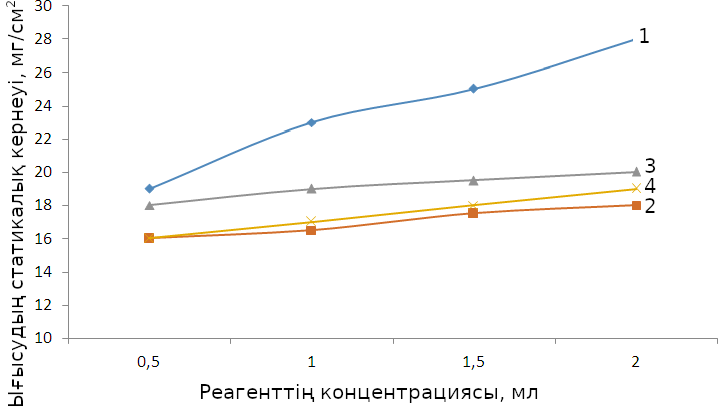
\includegraphics[width=0.8\textwidth]{media/gorn/image46}
	\caption*{}
\end{figure}


{\bfseries Ығысудың статикалық кернеуі, мг/см\textsuperscript{2}}

{\bfseries Реагенттің концентрациясы, мл}

{\bfseries 3 - сурет. Бұрғылау ерітіндісінің ығысуының статикалық кернеуінің
құрам компоненттерінің концентрациясына тәуелділігі}

\begin{multicols}{2}
Жоғарыда келтірілген тәуелділіктердің деректері зерттелетін жаңа
реагенттің концентрациясынан саз ерітінділерінің ығысу статикалық
кернеуі мен шартты тұтқырлығының өзгеруі іс жүзінде сызықтық
тәуелділікке ие екенін көрсетеді.

Айта кету керек, ұңғымаларды 800-1600 м аралықта бұрғылау кезінде
жоғарғы бөлігінде негізінен құмтастар басым болады, ал 1200 метрден
бастап сұр саздар, слюда, әртүрлі дәрежеде алеврит, кей жерлерде
опокоидты, сонымен қатар сидерит басым болады.

Бентонит сазының құрамын 10\% - ға дейін арттыру тұтқырлықтың
жоғарылауына себеп болады және судың бергіштігін төмендетеді, сонымен
қатар ұңғыма қабырғасының сапалы қабықшасының пайда болуына ықпал етеді.
Ығысудың статикалық кернеуі бұрғыланған тау жынысын бұрғылау ерітіндіде
ұстау үшін қажет талаптарға сәйкес келеді (3-сурет, 2-қисық). Жоғарыда
келтірілген композициялардың ішінен біз № 2 оңтайлы ерітінді ретінде
таңдадық (1-кесте), ол негізгі көрсеткіштер бойынша оң нәтиже көрсетті.
\end{multicols}

{\bfseries 1 - кесте. Бұрғылау ерітіндісінің технологиялық көрсеткіштері}

%% \begin{longtable}[]{@{}
%%   >{\raggedright\arraybackslash}p{(\linewidth - 8\tabcolsep) * \real{0.3942}}
%%   >{\centering\arraybackslash}p{(\linewidth - 8\tabcolsep) * \real{0.1558}}
%%   >{\centering\arraybackslash}p{(\linewidth - 8\tabcolsep) * \real{0.1624}}
%%   >{\centering\arraybackslash}p{(\linewidth - 8\tabcolsep) * \real{0.1360}}
%%   >{\centering\arraybackslash}p{(\linewidth - 8\tabcolsep) * \real{0.1516}}@{}}
%% \toprule\noalign{}
%% \begin{minipage}[b]{\linewidth}\centering
%% Бұрғылау ерітіндісінің құрамы, мл
%% \end{minipage} & \begin{minipage}[b]{\linewidth}\centering
%% тығыздық,
%% 
%% \emph{ρ}, кг/м\textsuperscript{3}
%% \end{minipage} & \begin{minipage}[b]{\linewidth}\centering
%% Шартты тұтқырлық, с
%% \end{minipage} & \begin{minipage}[b]{\linewidth}\centering
%% Сүзу,
%% 
%% см\textsuperscript{3}/30мин
%% \end{minipage} & \begin{minipage}[b]{\linewidth}\centering
%% ЫСК
%% 
%% мг /см\textsuperscript{2}
%% \end{minipage} \\
%% \midrule\noalign{}
%% \endhead
%% \bottomrule\noalign{}
%% \endlastfoot
%% №1. БС-- 6, ҰМТ -- 4, МПАА-0,5, су & 1100 & 25-30 & 6,0-6,5 &
%% 3-4/19-28 \\
%% №2. БС--4, ҰМТ --2, МПАА-0,8, су & 1050 & 30-35 & 3,7-4,8 & 2-3/16-18 \\
%% №3. БС-10, ҰМТ --5,МПАА-1,0, су & 1150 & 40-62 & 4,2-5,4 & 3-4/18-20 \\
%% №4. БС-- 8, ҰМТ --2, МПАА-1,0, су & 1200 & 50-54 & 4,0-5,0 &
%% 5-6/16-19 \\
%% \end{longtable}

\begin{multicols}{2}
Ұсынылған бұрғылау ерітіндісінің №2 оңтайлы ерітіндісі ұңғыма
қабырғасының қабықшасының сапасын қамтамасыз етеді, яғни бұрғылау
ерітіндісінің сіңірілуін төмендетеді, сонымен қатар су бергіштігін,
тұрақты тұтқырлық мәндерін және ығысудың статикалық кернеуін
төмендетеді. Айта кету керек, 1-кестеде келтірілген бұрғылау
ерітінділерінің құрамын шартты деп айтуға болады, өйткені ұңғыманың
келесі аймағына өту кезінде, яғни кондуктор, құрылым түзушіден басқа
қосымша химиялық реагенттер енгізіледі. Міндетті түрде беттік-активті
заттарды, майлағыш қоспаларын, КМЦ сүзілу төмендеткішін және т. б.
енгізу болып табылады.

Көрсету қабілеті 1х500 болатын жарық микроскопын қолдана отырып,
полимерлі реагенттің құрылымдық зерттеулерінің нәтижелері келтірілді.
Дистилденген май қышқылының (госсипол шайырының) сабындалған гудронымен
модификацияланған полиакриламид қоспасынан тұратын полимерлі реагенттің
сазды ерітіндісіне оптикалық зерттеулер жүргізілді (4-сурет).
\end{multicols}

%% \begin{longtable}[]{@{}
%%   >{\centering\arraybackslash}p{(\linewidth - 8\tabcolsep) * \real{0.3285}}
%%   >{\centering\arraybackslash}p{(\linewidth - 8\tabcolsep) * \real{0.0230}}
%%   >{\centering\arraybackslash}p{(\linewidth - 8\tabcolsep) * \real{0.3199}}
%%   >{\centering\arraybackslash}p{(\linewidth - 8\tabcolsep) * \real{0.0230}}
%%   >{\centering\arraybackslash}p{(\linewidth - 8\tabcolsep) * \real{0.3056}}@{}}
%% \toprule\noalign{}
%% \begin{minipage}[b]{\linewidth}\centering
%% 
%% \begin{figure}[H]
%% 	\centering
%% 	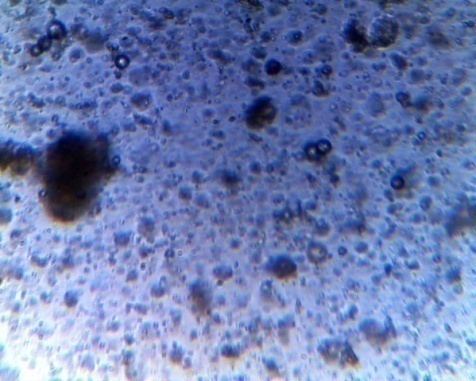
\includegraphics[width=0.8\textwidth]{media/gorn/image47}
%% 	\caption*{}
%% \end{figure}

%% \end{minipage} & \begin{minipage}[b]{\linewidth}\centering
%% \end{minipage} & \begin{minipage}[b]{\linewidth}\centering
%% 
%% \begin{figure}[H]
%% 	\centering
%% 	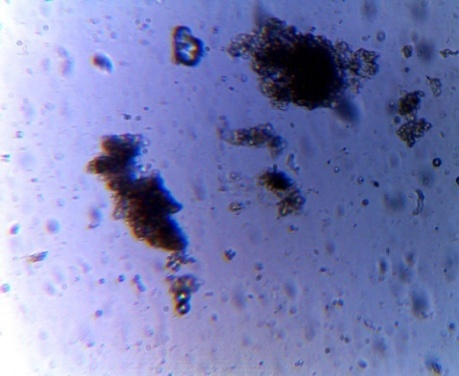
\includegraphics[width=0.8\textwidth]{media/gorn/image48}
%% 	\caption*{}
%% \end{figure}

%% \end{minipage} & \begin{minipage}[b]{\linewidth}\centering
%% \end{minipage} & \begin{minipage}[b]{\linewidth}\centering
%% 
%% \begin{figure}[H]
%% 	\centering
%% 	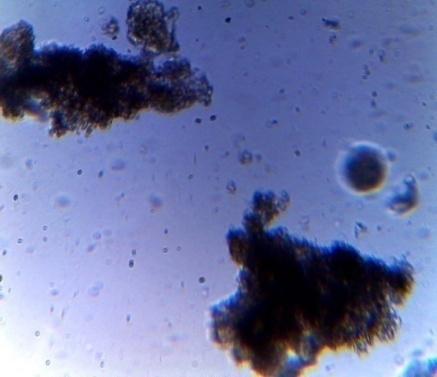
\includegraphics[width=0.8\textwidth]{media/gorn/image49}
%% 	\caption*{}
%% \end{figure}

%% \end{minipage} \\
%% \midrule\noalign{}
%% \endhead
%% \bottomrule\noalign{}
%% \endlastfoot
%% а & & б & & в \\
%% \end{longtable}

Белгіленулері: а- МПАА -0,5 мл; б) МПАА-1 мл; в) МПАА-1,5 мл.

{\bfseries 4 - сурет. Модификацияланған полимерлі реагенттің микросуреттері}

\begin{multicols}{2}
Жарық микроскопының көмегімен жүргізілген микроскопиялық зерттеулер,
үлгілер құрылымының келесі ерекшеліктерін анықтады. Жоғарыда берілген
микросуретте (4а-сурет) модификацияланған полимерлі реагенттің ұсақ
бөлшектері мен пішінсіз қосындылары бар полимерлі құрылым көрінеді.
Қызығушылық тудыратыны, 4б-суретте еритін бөлшектерден, орташа пішінсіз
аймақтардан тұратын әртүрлі полимерлі құрылым айқын байқалуы болды.4в
суретте еритін бөлшектерден, көптеген үлкен пішінсіз аймақтардан тұратын
әртүрлі полимерлі құрылым айқын байқалды.

Бұрғылау ерітіндісіндегі модификацияланған полимердің көмірсутектермен
және тау жыныстарымен өзара әрекеттесуі нәтижесінде молекулааралық
күштер, қатты бөлшектер -- су жүйесіндегі өзара әрекеттесу пайда болады
деп болжанады.

Алынған нәтижелер құрам түрінің, құрылымының, химиялық табиғаттының,
ингредиенттердің арақатынасының және олардың өзара әрекеттесу
механизмінің әсер ету заңдылықтарын анықтаудан тұратын практикалық
маңыздылыққа ие. Минералды және органикалық ингредиенттерді біріктіретін
композициялық химиялық реагенттерді құрудың негізгі физика-химиялық және
технологиялық ғылыми негіздері белгіленді.

{\bfseries Қорытынды.} Осылайша, жергілікті шикізат негізінде
модификацияланған полимерлі реагенттің композициялық химиялық
реагенттерін қолдану ұңғымаларды бұрғылау процесінде бұрғылау
ерітіндісінің тұрақтылығын арттырады. Суда жақсы еру қабілетіне
байланысты полимерлі компоненттер сабындалған шайырдың май қышқылдары
мен ұсақталған мақта талшығының құрамына байланысты бұрғылау
ерітіндісінің құрылымын нығайтуды қамтамасыз етеді. Алынған құрам
бұрғылау ерітіндісінің ығысуының статикалық кернеуіне, шартты
тұтқырлығына және майлауыш қасиеттеріне әсерін береді, бұл сөзсіз тау
жыныстарын бұзатын құралдың (қашаудың) қызмет ету мерзімін ұзартады.
Сонымен бірге су бергіштік коэффициентін төмендетуге және ұңғыма
қабырғасында пайда болған қабықшаның сапасын арттыруға, бұрғылау
ерітіндісін тұрақтандыруға ықпал етеді.

\emph{{\bfseries Қаржыландыру:}} бұл зерттеулер Қазақстан Республикасы
Ғылым және жоғары білім министрлігінің Ғылым комитетінің (ВR24992809)
қолдауымен жүргізілді.
\end{multicols}

\begin{center}
{\bfseries Әдебиеттер}
\end{center}

\begin{references}
1. Каукенова А.С. Перспективы нефтегазоносности в Южно-Торгайском
бассейне //Геология и разведка месторождений
углеводородов.-2020.-Vol.(3).-C.38-45. DOI
10.32454/0016-7762-2020-63-3-38-45

2. Конесев Г.В., Аксенова Н.А., Овчинников В.П. Технология бурения
нефтяных и газовых скважин. В 5 томах. Т.2 : учебник для студентов
вузов. -Тюмень: Тюменский индустриальный университет, 2017. -560 c. ISBN
978-5-9961-1330-9

3. Рябов Н.И. Методы предупреждения и ликвидации поглощений бурового
раствора при бурении нефтяных и газовых скважин. Самара, 2003. -- 64 с.

4. Ишмухамедова Н.К. Разработка и регулирование термосолеустойчивых
составов малоглинистых и полимерных растворов для бурения нефтяных и
газовых скважин: 25.00.15 «Технология бурения и освоения скважин»:
автореферат диссертации на соискание ученой степени доктора технических
наук / Ишмухамедова Насима Кенжебаевна; Атырауский институт нефти и
газа. -- Атырау, 2010. с.37-44.

5. RyenCaenn, George R., in Composition and Properties of Drilling and
Completion Fluids (Seventh Edition).2015,7(2), 63--29. ISBN
9780123838599

6. Alaskar MN, Ames MF, Connor ST, Liu C, Cui Y, Li K, et al.
Nanoparticle and microparticle flow in porous and fractured media-an
experimental study // SPEJ. -2012. --Vol.17(4). --P.1160-1171. DOI
10.2118/146752-pa.

7. Мартынов Н.Н., Заливин В.Г. Технология ликвидации поглощений бурового
раствора при бурении в интервалах трапповых интрузий // Известия
Сибирского отделения Секции наук о Земле Российской академии
естественных наук. Геология, разведка и разработка месторождений
полезных ископаемых. -2018. --Vol.41(4). -C.107--117. DOI
10.21285/2541-9455-2018-41-4-107-117

8. Минибаев В.В., Ильин И.А., Пестерев С.В. Эффективность полисахаридных
реагентов в буровых растворах различной степени минерализации среды //
Бурение и нефть. -- 2009. -- № 10. -- C.44-46.

9. Умедов Ш. Х. Разработка эффективных составов промывочных жидкостей
для борьбы с осложнениями при бурении нефтяных и газовых скважин: дисс.
... доктора технических наук, 05.15.10 -- Технология бурения и освоения
скважин. Ташкент -- 2017. -213 с.

10. Надиров К.С., Бимбетова Г.Ж., Сакибаева С.А., Тасанбаева Н.Е.,
Тортбаева Д.Р. Стабилизатор буровых растворов // Нефть и газ. -2007.
-№3. -C.26-29.

11. Патент 27482 РК, МПК С09К 8/34 (2006.01) Модифицированный буровой
раствор /Бондаренко В.П, Надиров К.С., Бимбетова Г.Ж. {[}и др.{]}. -№
2012/1022.1; заявл.05.10.2012; опубл.15.10.2013; Бюл. №10.
\end{references}

\begin{center}
{\bfseries References}
\end{center}

\begin{references}
1. Kaukenova A.S. Perspektivy neftegazonosnosti v Juzhno-Torgajskom
bassejne // Proceedings of Higher Educational Establishments: Geology
and Exploration. -- 2020. --Vol. (3). -C.38-45. DOI
10.32454/0016-7762-2020-63-3-38-45 {[}in Russian{]}

2. Konesev G.V., Aksenova N.A., Ovchinnikov V.P. Tehnologija burenija
neftjanyh i gazovyh skvazhin. V 5 tomah. T.2 : uchebnik dlja studentov
vuzov. -Tjumen': Tjumenskij
industrial' nyj universitet, 2017. -560 c. ISBN
978-5-9961-1330-9 {[}in Russian{]}

3. Rjabov N.I. Metody preduprezhdenija i likvidacii pogloshhenij
burovogo rastvora pri burenii neftjanyh i gazovyh skvazhin. Samara,
2003. -- 64 s. {[}in Russian{]}

4. Ishmuhamedova N.K. Razrabotka i regulirovanie termosoleustojchivyh
sostavov maloglinistyh i polimernyh rastvorov dlja burenija neftjanyh i
gazovyh skvazhin: 25.00.15 «Tehnologija burenija i osvoenija skvazhin»:
avtoreferat dissertacii na soiskanie uchenoj stepeni doktora
tehnicheskih nauk / Ishmuhamedova Nasima Kenzhebaevna; Atyrauskij
institut nefti i gaza. -- Atyrau, 2010. s.37-44. {[}in Russian{]}

5. RyenCaenn, George R., in Composition and Properties of Drilling and
Completion Fluids (Seventh Edition).2015,7(2), 63--29. ISBN
9780123838599

6. Alaskar MN, Ames MF, Connor ST, Liu C, Cui Y, Li K, et al.
Nanoparticle and microparticle flow in porous and fractured media-an
experimental study // SPEJ. -2012. --Vol.17(4). --P.1160-1171. DOI
10.2118/146752-pa.

7. Martynov N.N., Zalivin V.G. Tehnologija likvidacii pogloshhenij
burovogo rastvora pri burenii v intervalah trappovyh intruzij //
Izvestija Sibirskogo otdelenija Sekcii nauk o Zemle Rossijskoj akademii
estestvennyh nauk. Geologija, razvedka i razrabotka mestorozhdenij
poleznyh iskopaemyh. -2018. --Vol.41(4). -C.107--117. DOI
10.21285/2541-9455-2018-41-4-107-117 {[}in Russian{]}

8. Minibaev V.V., Il' in I.A., Pesterev S.V.
Jeffektivnost'{} polisaharidnyh reagentov v burovyh
rastvorah razlichnoj stepeni mineralizacii sredy // Burenie i
neft'. -- 2009. -- № 10. -- C.44-46. {[}in Russian{]}

9. Umedov Sh. H. Razrabotka jeffektivnyh sostavov promyvochnyh
zhidkostej dlja bor' by s oslozhnenijami pri burenii
neftjanyh i gazovyh skvazhin: diss. ... doktora tehnicheskih nauk,
05.15.10 -- Tehnologija burenija i osvoenija skvazhin. Tashkent -- 2017.
-213 s. {[}in Russian{]}

10. Nadirov K.S., Bimbetova G.Zh., Sakibaeva S.A., Tasanbaeva N.E.,
Tortbaeva D.R. Stabilizator burovyh rastvorov // Neft'{}
i gaz. -2007. -№3. -C.26-29. {[}in Russian{]}

11. Patent 27482 RK, MPK S09K 8/34 (2006.01) Modificirovannyj burovoj
rastvor /Bondarenko V.P, Nadirov K.S., Bimbetova G.Zh. {[}i dr.{]}. -№
2012/1022.1; zajavl.05.10.2012; opubl.15.10.2013; Bjul. №10. {[}in
Russian{]}
\end{references}

\begin{authorinfo}
\emph{{\bfseries Авторлар туралы мәліметтер}}

Бесбаева Н.А. - PhD докторанты,М.Әуезов атындағы Оңтүстік Қазақстан
университеті, Шымкент, Қазақстан, е-mail:besbaeva.nursulu@mail.ru;

Бимбетова Г.Ж.- техника ғылымдарының кандидаты, профессор, Оңтүстік
Қазақстан университеті, Шымкент, Қазақстан, е-mail:


Надиров К.С.- химия ғылымдарының докторы, профессор,М.Әуезов атындағы
Оңтүстік Қазақстан университеті, Шымкент, Қазақстан, е-mail:


Жантасов М.Қ. - техника ғылымдарының кандидаты, профессор, М.Әуезов
атындағы Оңтүстік Қазақстан университеті, Шымкент, Қазақстан, е-mail:


Отарбаев Н.Ш.- PhD, аға оқытушы, М.Әуезов атындағы Оңтүстік Қазақстан
университеті, Шымкент, Қазақстан, е-mail:
\href{mailto:otarbaevn@mail.ru}{}

\emph{{\bfseries Information about the authors}}

Besbaeva N.A. - PhD doctoral student, M. Auezov South Kazakhstan
University, Shymkent, Kazakhstan, е-mail:besbaeva.nursulu@mail.ru;

Bimbetova G.Zh. - Candidate of technical Sciences, Professor, M. Auezov
South Kazakhstan University, Shymkent, Kazakhstan, е-mail:


Nadirov K.S. - Doctor of chemical Sciences, Professor, M. Auezov South
Kazakhstan University, Shymkent, Kazakhstan, е-mail:


Zhatasov M.K.- Candidate of technical Sciences, Professor, Shymkent,
Kazakhstan, е-mail:


Otarbaev N.Sh.\textsuperscript{-} PhD, senior lecturer, M. Auezov South
Kazakhstan University, Shymkent, Kazakhstan, е-mail:
\href{mailto:otarbaevn@mail.ru}{}
\end{authorinfo}
